\documentclass[14pt, oneside]{altsu-report}

\worktype{Отчёт по <<Производственная практика: технологическая (проектно-технологическая) практика>> на тему:}
\title{Разработка игры Pac-man на языке программирования Python}
\author{М.\,А.~Давыдов}
\groupnumber{5.205-1}
\GradebookNumber{1337}
\supervisor{И.\,А.~Шмаков}
\supervisordegree{ст.пр}
\ministry{Министерство науки и высшего образования}
\country{Российской Федерации}
\fulluniversityname{ФГБОУ ВО Алтайский государственный университет}
\institute{Институт цифровых технологий, электроники и физики}
\department{Кафедра вычислительной техники и электроники}
\departmentchief{В.\,В.~Пашнев}
\departmentchiefdegree{к.ф.-м.н., доцент}
\shortdepartment{ВТиЭ}
\abstractRU{В отчёте содержатся сведения о курсовой работе.

Курсовая работа заключается в создании кроссплатформенной программы, представляющей собой игру Pac-man.

В отчёте приведено описание используемой библиотеки, инструментария и системы контроля версий для написания программы на языке программирования Python3.

Также в отчёте приведены общие сведения об игре Pac-man.

Наряду с этим представлены проверка работспособности программы, блок-схема, полный код программы.}
\abstractEN{The report contains information about the course work.

The course work is to create a cross-platform program that is a Pac-man game.

The report describes the library, tools, and version control system used to write a program in the Python3 programming language.

The report also provides general information about the Pac-man game.

Along with this, a program health check, a flowchart, and the full program code are presented.}
\keysRU{программа, игра, пакман, алгоритм, кроссплатформенная программа}
\keysEN{program, game, pacman, algorithm, cross-platform program}

\date{\the\year}

% Подключение файлов с библиотекой.
\addbibresource{graduate-students.bib}

% Пакет для отладки отступов.
%\usepackage{showframe}

\begin{document}
\maketitle

\setcounter{page}{2}
\makeabstract
\tableofcontents

\chapter*{Введение}
\phantomsection\addcontentsline{toc}{chapter}{ВВЕДЕНИЕ}

\textbf{Актуальность:}
Технологическая (проектно-технологическая) практика заключается в приобретении студентами практических навыков и знаний в области проектирования и разработки программного обеспечения (ПО). Ещё практика позволяет закрепить и расширить теоретические знания студентов, полученных в процессе обучения, приобрести практические навыки в сфере разработки ПО, а также развить навык самостоятельного принятия решений задач. Также практика позволяет студентам познакомиться с процессом разработки программного обеспечения с самого начала, от анализа требований до внедрения готового продукта.

Разработка кроссплатформенной программы на языке программирования Python может послужить хорошим стимулом как для более глубокого изучения программирования, так и для понимания сборки программы под различные платформы.

Разработка игры в жанре <<Аркада>> позволяет сформировать представление о самом её <<скелете>>, о её графической составляющей, о правильном построении алгоритмов.

По сей день аркадные игры популярны среди игроков различных возрастов, так как они позволяют скоротать время в поездке или, например, на лекции или на скучном собеседовании. Разработка такой игры может быть актуальной, так как на рынке существует множество игр этого жанра, но мало качественных проектов, которые могут предложить что-то новое и интересное.

\textbf{Цель:}
Создать кроссплатформенную игру Pac-man с использованием языка программирования Python3 и библиотеки PySDL2.

\textbf{\label{zadachi}Задачи:}
\begin{enumerate}
	\item Изучить графическую библиотеку PySDL2.
	\item Изучить алгоритмы игры Pac-man.
	\item Научиться выставлять собственную частоту кадров игровой области.
	\item Научиться работать в среде разработки программного обеспечения Microsoft VS Code.
	\item Разобраться во взаимодействии компьютерной графики с аппаратным или программным обеспечением.
	\item Изучить принцип ООП в Python.
	\item Закрепить навыки в работе с системой компьютерной вёрстки \TeX и его расширения \XeTeX.
\end{enumerate}

% Подключение первой главы (теория):
\chapter{\label{ch:ch01}ОБЗОР ИНСТРУМЕНТАРИЯ ДЛЯ СОЗДАНИЯ КОМПЬЮТЕРНОЙ ИГРЫ}

\section{\label{sec:ch01/sec01}Техническое задание.}
\begin{enumerate}
	\item Кроссплатформенное приложение, способное запускаться на операционных системах Windows и GNU/Linux.
	\item Написание игры Pac-Man на языке программирования Python3.
	\item Использование графической библиотеки PySDL2.
	\item Возможность выбора карты или генерация карты в игре Pac-Man.
	\item Возможность выбора количества врагов в игре Pac-Man.
	\item Движение призраков не так важно, главное --- чтобы они преследовали пакмана.
	\item Наличие в игре кнопки <<Помощь>>, при нажатии на которую выводится информация об игре(например, её управлении), а также реферат об этой игре.
\end{enumerate}

\section{\label{sec:ch01/sec02}Графическая библиотека.}
Для создания кроссплатформенной программы на языке программирования Python3 была использована графическая библиотека PySDL2~\cite{pypiRUENpysdl2,docENpysdl2}.

\textbf{PySDL2}~\label{pysdl2} --- это чистая оболочка Python для библиотек \textit{SDL2, SDL2\_mixer, SDL2\_image, SDL2\_ttf и SDL2\_gfx}. Вместо того, чтобы полагаться на код С, она использует
встроенный модуль \textbf{ctypes} для взаимодействия с SDL2 и предоставляет простые классы Python и оболочки для общих функций SDL2.

PySDL2 состоит из двух пакетов: \textbf{sdl2}, который представляет собой простую API-оболочку 1:1 вокруг API SDL2, и \textbf{sdl2.ext}, который предлагает расширенные функциональные возможности для \textbf{sdl2}.

Пакет \textbf{sdl2} реализован таким образом, что его можно легко интегрировать и развертывать с собственными программными проектами.

Модуль \textbf{sdl2.ext} предоставляет богатый набор модулей, классов и функций для создания игр и других приложений с использованием PySDL2.

Цель модуля \textbf{sdl2.ext} --- обернуть часто используемые части API SDL2 более дружественным и питоническим способом, уменьшая необходимость для разработчиков разбираться в тонкостях работы \textbf{ctypes} и делая создание программ PySDL2 более простым и увлекательным.
Кроме того, этот модуль предоставляет ряд классов шаблонов и служебных функций для работы с цветами, событиями ввода, файловыми ресурсами и т. д.


\section{\label{sec:ch01/sec03}Инструментарий.}
Для написания отчёта с помощью системы компьютерной верстки в \TeX была использована IDE TexStudio~\cite{texRUtexstud,texENtexstud}, а также дистрибутив Tex Live~\cite{texRUtexlive}.

Для написания кода программы была использована IDE Microsoft Visual Studio Code~\cite{vscodeEN}.

Для работы с изображениями, используемых в ходе разработки программы, был использован графический редактор Adobe Photoshop 2023~\cite{adobeRU}.

Для хранения проекта была выбрана система контроля версия GitHub~\cite{wikiRUGitHub}.

Проверка работоспособности и сборка программы выполнялась на системе:
	\begin{itemize}
		\item \textbf{OC}: \textit{Windows 10}
		\item \textbf{ЦП}: \textit{AMD FX-6300}
		\item \textbf{ОЗУ}: \textit{8gb}
		\item \textbf{Видеокарта}: \textit{NVIDIA GeForce GTX 1050}
	\end{itemize}
	

\section{\label{sec:ch01/sec04}Игра Pac-Man.}
\subsection{\label{subsec:ch01/sec04/subsec01}История игры.}
\textbf{Pac-Man} --- аркадная видеоигра, разработанная японской компанией Namco и вышедшая в 1980 году~\cite{pacmanRU}.

В конце 1970-х из-за успеха игры Space Invaders рынок видеоигр сосредоточился на создании аркадных шутемапов и привлекал к себе сугубо мужскую аудиторию. Сотрудник Namco Тору Иватани хотел сделать игру, которая понравилась бы всем, в особенности девушкам, и в качестве основной темы своей работы выбрал еду. В Японии созданная игра получила название Puck-Man, но при локализации в США компания Midway изменила название на Pac-Man, считая, что при оригинальном названии дети могли бы закрасить середину буквы «P», превратив её в «F», и сделать слово обсценным.

После выхода в Японии игра была принята хорошо, но не стала популярной. В Америке же аудитория была впечатлена отсутствием в аркаде насильственного мотива, что привлекло в том числе женскую аудиторию и помогло заработать лояльность родителей к видеоигре. Всё это обеспечило популярность Pac-Man среди людей разных возрастов и профессий, породив повышенный интерес к игре и сделав Пакмана первой звездой видеоигр. Такой успех вдохновил разработчиков на создание более разнообразных игр, в том числе с отсутствием насилия.

Благодаря популярности игра портировалась и переиздавалась на множество платформ, среди которых особую известность получила версия Pac-Man для Atari 2600. Из-за своего плохого качества она стала одним из символов кризиса видеоигр 1983 года. Pac-Man дала начало одноимённой серии игр, в которой вышло множество продолжений на различных платформах, включая аркадные автоматы, домашние игровые системы, компьютеры и мобильные телефоны. Помимо этого, вышло множество клонов, подражаний и нелегальных копий игры.

\subsection{\label{subsec:ch01/sec04/subsec02}Правила игры.}
Экран игры представляет собой лабиринт, коридоры которого заполнены точками.

Задача игрока --- управляя Пакманом, съесть все точки в лабиринте, избегая встречи с привидениями, которые гоняются за героем.

В начале каждого уровня призраки находятся в недоступной Пакману прямоугольной комнате в середине уровня, из которой они со временем освобождаются. Если привидение дотронется до Пакмана, то его жизнь теряется, призраки и Пакман возвращаются на исходную позицию, но при этом прогресс собранных точек сохраняется. Если при столкновении с призраком у Пакмана не осталось дополнительных жизней, то игра заканчивается. После съедения всех точек начинается новый уровень в том же лабиринте. По бокам лабиринта находятся два входа в один туннель, при вхождении в который Пакман и призраки выходят с другой стороны лабиринта.

Всего в лабиринте находятся 240 маленьких точек и 4 большие, известные как энерджайзеры . За съедение маленькой точки даётся 10 очков, а за съедение энерджайзера — 50. Таким образом, в общей сложности все точки в лабиринте стоят 2600 очков. При съедении Пакманом энерджайзера призраки в лабиринте на короткое время входят в режим испуга, резко меняют направление движения и перекрашиваются в синий цвет. За это время Пакман способен съесть призраков посредством столкновения с ними, которое безопасно. От съеденного привидения остаются только глаза, которые возвращаются в центр лабиринта, где призрак вновь оживает и отправляется в погоню за Пакманом. За съедение первого призрака после получения энерджайзера даётся 200 очков. За съедение каждого следующего привидения при эффекте того же энерджайзера даётся в два раза больше: 400, 800 и 1600 соответственно. Таким образом, при съедении всех призраков после каждого эффекта энерджайзера игрок может заработать за один уровень 12 000 очков.

\subsection{\label{subsec:ch01/sec04/subsec03}Поведение призраков.}
\begin{itemize}
	\item Красный призрак Шэдоу по прозвищу Блинки. В режиме преследования использует как цель ту клетку, в которой находится Пакман. Блинки, в отличие от других привидений, увеличивает свою скорость преследования относительно первоначальной дважды за уровень в зависимости от количества съеденных точек. Если точек осталось мало, то он меняет целевую клетку в режиме рассеивания на квадрат, в котором находится Пакман, и так гоняется за героем в двух режимах.
	\item Розовый призрак Спиди по прозвищу Пинки. В качестве цели при преследовании использует точку, находящуюся на четыре клетки впереди Пакмана. Однако из-за ошибки переполнения при движении Пакмана вверх Пинки использует в качестве цели квадрат, находящийся на четыре клетки вверх и на четыре влево от Пакмана.
	\item Голубой призрак Башфул по прозвищу Инки. Использует самый сложный алгоритм преследования: для определения направления движения строится отрезок, один из концов которого определяется положением Блинки, а середина находится на 2 клетки перед Пакманом. Второй конец отрезка --- искомая целевая точка. Получившуюся точку сложно предсказать, поэтому Инки считается самым опасным привидением. Из-за ошибки переполнения, аналогичной в поведении Пинки, во время движения Пакмана вверх целевая клетка Инки это две клетки вверх и две влево от Пакмана.
	\item Оранжевый призрак Поки по прозвищу Клайд. Если Клайд находится дальше 8 клеток от Пакмана, то он использует в качестве цели самого Пакмана, как Блинки. Если же Пакман ближе 8 клеток, то Клайд стремится к левому нижнему углу, как при рассеивании.
\end{itemize}



% Подключение второй главы (практическая часть):
\chapter{\label{ch:ch02}ГЛАВА 2. ЭТАПЫ РАЗРАБОТКИ ИГРЫ. ПРОВЕРКА РАБОТОСПОСОБНОСТИ ПРОГРАММЫ.}

\section{\label{sec:ch02/sec01}Этапы разработки игры.}

\subsection{\label{subsec:ch02/sec01/sub01}Установка собственной частоты кадров.}
\textbf{FPS} --- частота кадров в секунду, демонстрируемая игрой.

Собственная частота кадров --- это первая проблема, с которой пришлось столкнуться при написании кода игры. Например, в библиотеке pygame есть функция \textbf{Clock()},
благодаря которой можно задать собственный FPS. В библиотеке PySDL2 такой функции нет.Для решения данной проблемы была попытка в использовании модуля Pygame\_sdl2.

\textbf{Pygame\_sdl2} --- это повторная реализация API Pygame с использованием SDL2 и связанных библиотек, выпущенная под лицензией Zlib~\cite{pgsdl2EN}.
После установки Pygame\_sdl2, попытка увеличить FPS не увенчалась успехом: модуль просто не работал. Интерпретатор попросту не смог его импортировать в код игры.

И только на этапе тестирования была выявлена причина медленной работы программы. 
Подробнее об этом (см. \textbf{\textsc{Взаимодействие компьютерной графики с аппаратным или программным обеспечением}}~\ref{subsec:ch02/sec01/sub02}).

\subsection{\label{subsec:ch02/sec01/sub02}Взаимодействие компьютерной графики с аппаратным или программным обеспечением.}
Как было сказано выше, проблема установки собственной частоты кадров решилась только на этапе тестирования. На этапе тестирования было замечено, что в режиме <<холостого хода>>
приложение очень стремительно потребляла оперативную память, и в итоге в терминал выводилась ошибка о выходе за пределы памяти (Out of memory). Было нетрудно догадаться,
что FPS было низким из-за большого потребления памяти.

Вообще существовала первая версия данной библиотеки для C/C++ и называлась просто: SDL. Эта версия библиотеки использовала использовала процессор для создания графических объектов.
Для создания графики на этой библиотеке использовался метод \textbf{SDL\_Surface}, который создавал поверхность, на которой можно было <<рисовать>>. А так как обработка всех графических объектов выполнялась процессором, это озночало то, что приложение может сильно тормозить, в зависимости от габаритов объектов (их количества, цветовой палитры и т.д.).

Вторая же версия, которая в частности использовалась для создания игры Pac-man, называется просто: SDL2. В ней, для облегчения работы процессора, используется метод \textbf{SDL\_Renderer},
который предназначен уже для ускорения с помощью видеокарты и прочих компонентов ПК. Помимо этого, в эту версию библиотеки была добавлена возможность для работы с OpenGL, Vulkan, DirectX.
Данный метод позволяет создавать спрайты (графический объект в компьютерной графике). Так вот проблема частоты кадров была именно в этом.

Изначально для создания текстур использовался метод \textbf{TEXTURE}, который загружал картинки и текст и переносл их в контекст рендера, не преобразовывая их в спрайты. Из-за этого было большое
потребление памяти, а следовательно, и маленькая частота кадров. В конечном итоге метод \textbf{TEXTURE} был замёнен на метод \textbf{SpriteFactory}, который загружает картинки и текст в контекст рендера, преобразовывая их в спрайты. В результате получилось, что программа перестала потреблять оперативную память, а следовательно повысилась частота кадров, и игра стала работать намного плавнее.

Также при тестирования игры на компьютерах с различными комплектующими было замечено, что, чем мощнее комплектующие, тем быстрее работает игра. Возможно это зависит от типа оперативной памяти, процессора, видеокарты или от всего вместе.

\subsection{\label{subsec:ch02/sec01/sub03}Создание меню игры.}
Игровое меню --- первое, с чего начиналось создание игры. Для игрового меню был создан класс \textit{ImageButton}, который содержит методы: \textit{\_\_init\_\_}, в котором объявляются переменные для цвета, текстур, самих кнопок и их расположения на экране; \textit{play\_sound}, предназначенный для воспроизведения звука при нажатии на кнопку; \textit{show\_menu}, который отрисовывает кнопки главного меню; \textit{show\_help}, который отрисовывает экран раздела <<Помощь>>; \textit{show\_select}, который отрисовывает экран выбора количества призраков и карты; \textit{render\_clean}, который очищает контекст рендера при нажатии на какую-либо из кнопок (см. \textbf{\textsc{ПРИЛОЖЕНИЕ}} на стр.~\pageref{code:menu} строки 5-71).

\subsection{\label{subsec:ch02/sec01/sub04}Создание карты.}
Изначально карта представляет собой двумернуый массив, заполненный числами от 0 до 9 (см. \textbf{\textsc{ПРИЛОЖЕНИЕ}} на стр.~\pageref{code:b1},~\pageref{code:b2},~\pageref{code:b3}).

В файле \textit{level.py} импортируются файлы с этими массивами (см. \textbf{\textsc{ПРИЛОЖЕНИЕ}} на стр.~\pageref{code:level} строки 3-5).

Функция \textit{selected\_level} предназначена для возврата в главную функцию программы полной копии карты (массива), которую выбирает игрок. В дальнейшем это понадобится не только для первоначальной отрисовки карты, но и для перерисовки карты в случае победы/поражения (см. \textbf{\textsc{ПРИЛОЖЕНИЕ}} на стр.~\pageref{code:level} строки 9-19).

Функция \textit{draw\_board} предназначена, собственно, для отрисовки карты в контекст рендера (см. \textbf{\textsc{ПРИЛОЖЕНИЕ}} на стр.~\pageref{code:level} строки 21-56). Данная функция пробегает по столбцам и строкам массива. В зависимости от числа она добавляет в контекст рендера по координатам соответствующий элемент, отрисовка которого происходит по правилу ниже (см. рисунок~\ref{fig1}).
\begin{figure}[H]
	\centering
	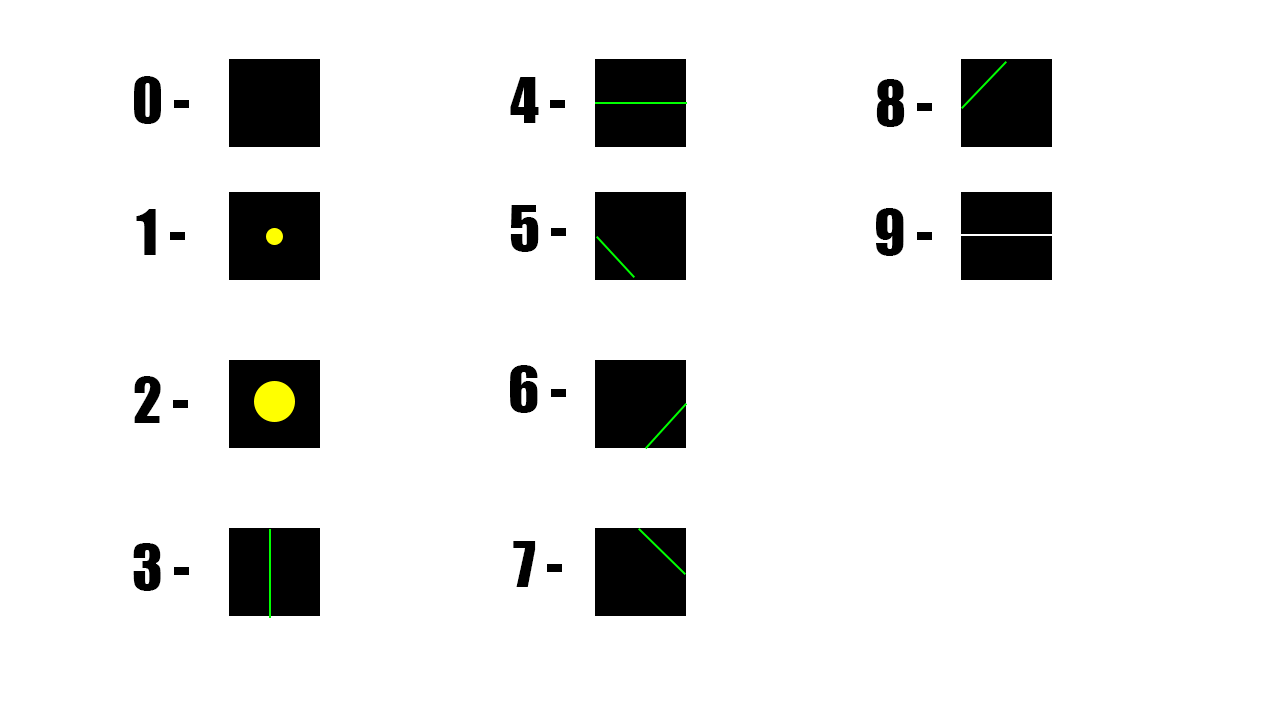
\includegraphics[width=1\linewidth]{images/карта.png}
	\caption{Правило отрисовки карты.}
	\label{fig1}
\end{figure}

\subsection{\label{subsec:ch02/sec01/sub05}Создание пакмана и функций для работы с ним.}
Изначально для пакмана создавался класс, но после неудачных попыток по возвращению некоторых переменных в главную функцию программы (пакман не двигался или двигался только вправо/влево), было решено использовать обычные функции.

Функция \textit{draw\_player} предназначена для добавления текстур пакмана в контекст рендера в зависимости от его направления и координат. Также в функцию передаётся переменная-счётчик, благодаря которой пакман как бы открывает и закрывает рот с каждой итерацией главного игрового цикла (см. \textbf{\textsc{ПРИЛОЖЕНИЕ}} на стр.~\pageref{code:player} строки 13-29).

Функция \textit{check\_position} предназначена для проверки на столкновение пакмана со стенкой лабиринта в зависимости от его направления и координат центра персонажа (см. \textbf{\textsc{ПРИЛОЖЕНИЕ}} на стр.~\pageref{code:player} строки 31-79). В главную функцию игры она возвращает значения: разрешено ли дальнейшее движение в указанном направлении или нет?

Функция \textit{move} предназначена для движения пакмана в зависимости от его направления и разрешения движения в данном направлении. Скорость пакмана равна двум, движение осуществляется просто: к координате пакмана по оси X с каждой итерацией игрового цикла прибавляется значение скорости (т.е. когда пакман движется горизонтально), а когда пакман движется вертикально, то от координаты по оси Y отнимается значение скорости (см. \textbf{\textsc{ПРИЛОЖЕНИЕ}} на стр.~\pageref{code:player} строки 81-93).

Функция \textit{check\_target} предназначена для поедания точек и призраков пакманом. Если координата центра пакмана совпадает с 1 в массиве карты, то 1 заменяется на 0, и точка уже не отрисовывается (см. \textbf{\textsc{Создание карты}} на стр.~\pageref{subsec:ch02/sec01/sub04}), при этом значение счётчика увеличивается на 10 в соответствии с правилами игры (см. \textbf{\textsc{Правила игры}} на стр.~\pageref{subsec:ch01/sec04/subsec02}), а также воспроизводится звук поедания точки. Если координата центра пакмана совпадает с 2 в массиве карты, то 2 заменяется на 0, и энерджайзер уже не отрисовывается (см. \textbf{\textsc{Создание карты}} на стр.~\pageref{subsec:ch02/sec01/sub04}), при этом значение счётчика увеличивается на 50, призраки становятся уязвимы, начинается отсчёт времени действия энерджайзера в соответствии с правилами игры (см. \textbf{\textsc{Правила игры}} на стр.~\pageref{subsec:ch01/sec04/subsec02}), а также воспроизводится звук поедания точки. В главную функцию check\_target возвращает значение счётчика, статус энерджайзера, начало отсчёта времени действия энерджайзера, статус съеденного призрака (см. \textbf{\textsc{ПРИЛОЖЕНИЕ}} на стр.~\pageref{code:player} строки 95-113).

Функция \textit{draw\_counter} предназначена для отрисовки на экране количества очков, статуса энерджайзера, жизней пакмана и надписи в случае проигрыша или поражения (см. \textbf{\textsc{ПРИЛОЖЕНИЕ}} на стр.~\pageref{code:player} строки 115-132).

Блок функций \textit{get\_targets\_4 - get\_targets\_7} предназначен для взаимодействия координат пакмана с координатами призраков в зависимости от количества выбранных призраков игроком. Если энерджайзер активен и призраки не съедены, то они начинают беспорядочное движение, по сути как бы убегают от пакмана. Если энерджайзер активен и призраки съедены, то их глаза возвращаются в место их перерождения. Если энерджайзер активен и призраки переродились, то они выходят из своей <<коробки>> и продолжают преследование пакмана. Если же энерджайзер не активен и призраки не съдены, то они преследуют пакмана. В противном случае, если они были съедены после окончания действия энерджайзера, то их глаза возвращаются в место их перерождения (см. \textbf{\textsc{ПРИЛОЖЕНИЕ}} на стр.~\pageref{code:player} строки 134-559).

\subsection{\label{subsec:ch02/sec01/sub06}Создание призраков.}
В связи с тем, что по ТЗ требуется возможность выбора количества призраков, то исходя из таких задач был создан класс \textit{Ghost}. 

Метод \textit{\_\_init\_\_} предназначен для объявления переменных, которые представляют собой характеристики каждого из призраков: координаты, координаты центра, координаты для преследования пакмана (см. \textbf{\textsc{Создание пакмана и функций для работы с ним}} о блоке функций \textit{get\_targets\_4 - get\_targets\_7} на стр.~\pageref{subsec:ch02/sec01/sub05}), текстуры, идентификационный номер, хитбокс, статус: призрак жив, в <<коробке>>, энерджайзер активен (см. \textbf{\textsc{ПРИЛОЖЕНИЕ}} на стр.~\pageref{code:ghost} строки 7-28).

Метод \textit{draw\_ghost} предназначен для добавления текстур призраков контекст рендера в зависимости от его идентификационного номера и статуса (жив, съеден или энерджайзер активен). Также, после добавления текстур, данный метод создаёт хитбокс призрака и возвращает его в метод \textit{\_\_init\_\_} (см. \textbf{\textsc{ПРИЛОЖЕНИЕ}} на стр.~\pageref{code:ghost} строки 30-42).

Метод \textit{check\_collisions} предназначен для проверки столкновения призраков со стенкой, а также для движения в указанном направлении. Данный метод работает аналогично функции \textit{check\_position} для пакмана (см. \textbf{\textsc{Создание пакмана и функций для работы с ним}} о функции \textit{check\_position} на стр.~\pageref{subsec:ch02/sec01/sub05}). Единственное отличие в том, что на призраков ещё накладываются условия о состоянии их статуса: жив (выход из коробки и в дальнейшем он в неё не заходит), съеден (глаза возвращаются обратно в <<коробку>>) и в <<коробке>> ли он (перерождение). В конце своей работы метод возвращает информацию о разрешении движения в указанном направлении, а также статус: в <<коробке>> ли призрак, в метод \textit{\_\_init\_\_} (см. \textbf{\textsc{ПРИЛОЖЕНИЕ}} на стр.~\pageref{code:ghost} строки 44-121).

Блок методов \textit{move\_blinky - move\_clyde} предназначен для движения призраков. Движение определяется в зависимости от координат призраков, разрешения движения в данном направлении, а также от координат, которые получаются из блока функций \textit{get\_targets\_4 - get\_targets\_7} (см. \textbf{\textsc{Создание пакмана и функций для работы с ним}} о блоке функций \textit{get\_targets\_4 - get\_targets\_7} на стр.~\pageref{subsec:ch02/sec01/sub05}). Также призраки обладают разной скоростью в зависимости от статуса: жив --- скорость равна 2, испуган (энерджайзер активен) --- скорость равна 1, съеден (движение глаз) --- скорость равна 4. Ко всему прочему, призраки имеют разную модель передвижения. Так как по ТЗ не важно, как двигаются призраки, но всё равно была предпринята попытка сделать движение призраков исходя из правил их поведения (см. \textbf{\textsc{Поведение призраков}} на стр.~\pageref{subsec:ch01/sec04/subsec03}):
\begin{itemize}
	\item Движение Блинки (красного, метод \textit{move\_blinky}) выполняется следующим образом: он поворачивается при каждом столкновении со стенкой, в противном случае
	продолжает движение прямо (см. \textbf{\textsc{ПРИЛОЖЕНИЕ}} на стр.~\pageref{code:ghost} строки 123-235).
	\item Движение Инки (голубого, метод \textit{move\_inky}) выполняется следующим образом: он поворачивает в любой момент вверх и вниз, чтобы преследовать пакмана, но влево и вправо только при столкновении со стенкой (см. \textbf{\textsc{ПРИЛОЖЕНИЕ}} на стр.~\pageref{code:ghost} строки 237-365).
	\item Движение Пинки (розового, метод \textit{move\_pinky}) выполняется следующим образом: он поворачивает в любой момент влево и вправо, чтобы преследовать пакмана, но вверх и вниз только при столкновении со стенкой (см. \textbf{\textsc{ПРИЛОЖЕНИЕ}} на стр.~\pageref{code:ghost} строки 367-498).
	\item Движение Клайда (оранжевого, метод \textit{move\_clyde}) выполняется следующим образом: он разваорачивается тогда, когда это выгодно для преследования пакмана (см. \textbf{\textsc{ПРИЛОЖЕНИЕ}} на стр.~\pageref{code:ghost} строки 500-644).
\end{itemize}

В конце каждый из этих методов возвращает в главный цикл игры координаты призраков и значения их направлений (0 -- вправо, 1 -- влево, 2 -- вверх, 3 -- вниз).

\subsection{\label{subsec:ch02/sec01/sub07}Главная функция игры.}
В главной функции игры инициализируется графическая библиотека \textit{init(), quit()}. Всё, что требуется для игры, прописывается между этими командами.

До главного игрового цикла происходит создание окна игры, рендера для отрисовки текстур, инициализация аудиоканала, объявление фабричного класса для создания спрайтов (текстур), переменных для работы с функциями пакмана, призраков, меню и игры, а также загрузка текстур и создание экземпляра класса кнопок (см. \textbf{\textsc{ПРИЛОЖЕНИЕ}} на стр.~\pageref{code:main} строки 11-135).

Мною было принято решение передавать переменные в функции пакмана и т.п. из главного цикла, потому что, во-первых, их значения изменяются с каждой итерацией игрового цикла, во-вторых, текстуры нужно загружать однажды, чтобы избежать торможения игры, как и было сказано выше (см. \textbf{\textsc{Взаимодействие компьютерной графики с аппаратным или программным обеспечением}} на стр.~\pageref{subsec:ch02/sec01/sub02}).

Игровой цикл условно можно разделить на несколько блоков: работа с меню игры, работа с самой игрой, обработка событий (нажатие кнопок). 

В блоке работы с меню игры обрабатываются все действия игрока: нажатие на кнопки, смена экранов, выбор количества призраков и карты, возврат на предыдущий экран. Если вдруг пользователь выбрал не то количество призраков или не ту карту, то ему следует нажать кнопку <<Назад>> и повторить операцию выбора (см. \textbf{\textsc{ПРИЛОЖЕНИЕ}} на стр.~\pageref{code:main} строки 138-152, 1584-1631). 

В блоке работы с игрой выполняется следующее: в зависимости от выбора игроком количества призраков и карты, создаётся соответствующее игровое поле. В начале отрабатывают счётчики, благодаря которым пакман и призраки не двигаются. Как только они начинают свои движения, то их первоначальные характеристики начинают изменяться с каждой итерацией и передаются в функции, описанные выше. 

Например, разберу случай выбора 4-ёх призраков и 1-ой карты. Как только в главном меню сделан выбор, то в функцию \textit{selected\_level} передаётся булева переменная в соответствии с выбранным уровнем, а она загружает и возвращает соответствующий. Далее происходит отработка счётчиков, описанных выше. Затем отрисовывается лабиринт со всеми точками. Потом создаётся хитбокс пакмана, который также зависит от его изменяющихся координат. Так как было выбрано 4 призрака, создается 4 экземпляра класса \textit{Ghost}, в которые передаются все переменные для работы с призраками, которые в свою очередь тоже меняются с каждой итерацией и ситуацией на игровом поле; выполняется вызов функций \textit{draw\_counter, get\_targets\_4, check\_position}, которые были описаны выше. Затем вызываются методы для движения пакмана и призраков. Управление пакманом осуществляется за счёт стрелок на клавиатуре (при нажатии на стрелку изменяется соответствующая переменная для направления движения, а уже в зависимости от направления проверяется проверка: разрешено ли туда двигаться или нет). При этом пакман проходит через тоннель и появляется с другой стороны лабиринта. Далее выполняется проверка на столкновение хитбоксов пакмана и призраков в зависимости от разных ситуаций:
\begin{itemize}
	\item Энерджайзер не активен -- при столкновении пакмана с призраком отнимается жизнь, все переменные принимают своё первоначальное значение, но съеденные точки не отображаются, счётчик не обнуляется.
	\item Энерджайзер активен -- пока другие призраки испуганы, при столкновении пакмана с перерождённым призраком отнимается жизнь, все переменные принимают своё первоначальное значение, но съеденные точки не отображаются, счётчик не обнуляется. При этом столкновение пакмана и глаз ни к чему не приводит.
	\item Энерджайзер активен -- если нет перерождённых или съеденных призраков (их глаз), пакман сталкивается с испуганным призраком, он превращатся в глаза, возвращается в <<коробку>> и перераждается.
\end{itemize}
В зависимости от типа столкновений изменяются скорости призраков, описание которых приведено выше (см. \textbf{\textsc{Создание призраков}} на стр.~\pageref{subsec:ch02/sec01/sub06}). Если жизней не осталось, то объекты останавливаются, выводится сообщении о проигрыше, и после нажатия на кнопку <<SPACE>> происходит перезапуск игры. Аналогично и для выигрыша, только проверяется условие на наличие точек в игровом поле.
 
Далее все проверки повторяются с каждой итерацией игрового цикла, начиная с первого пункта. Аналогично происходит для разного количества призраков и другой карты (см. \textbf{\textsc{ПРИЛОЖЕНИЕ}} на стр.~\pageref{code:main} строки 154-1574, 1638-1707).

Помимо всего в начале игры, при поедании пакманом точек и призраков, их перерождении воспроизводится звук.

С каждой итерацией игрового цикла рендер показывается и очищается, окно обновляется. Таким образом и происходит смена кадров.

\subsection{\label{subsec:ch02/sec01/sub08}Блок-схема.}
Поскольку выше я описал принцип работы программы, то решил сделать блок-схему более абстрагированной ввиду громоздкости кода программы. Блок-схема, описывающая алгоритмы и процессы в программе, приведена на рисунках~\ref{fig7}~\ref{fig8}.
\begin{figure}[H]
	\centering
	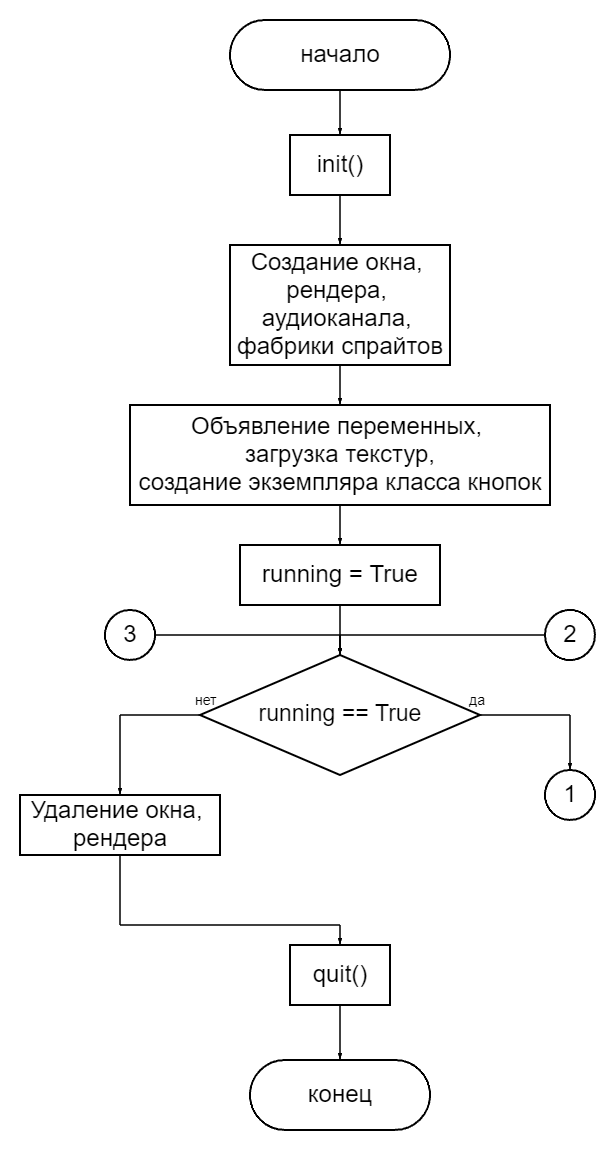
\includegraphics[width=0.8\linewidth]{images/flow1.png}
	\caption{Блок-схема алгоритма программы.}
	\label{fig7}
\end{figure}
\begin{figure}[H]
	\centering
	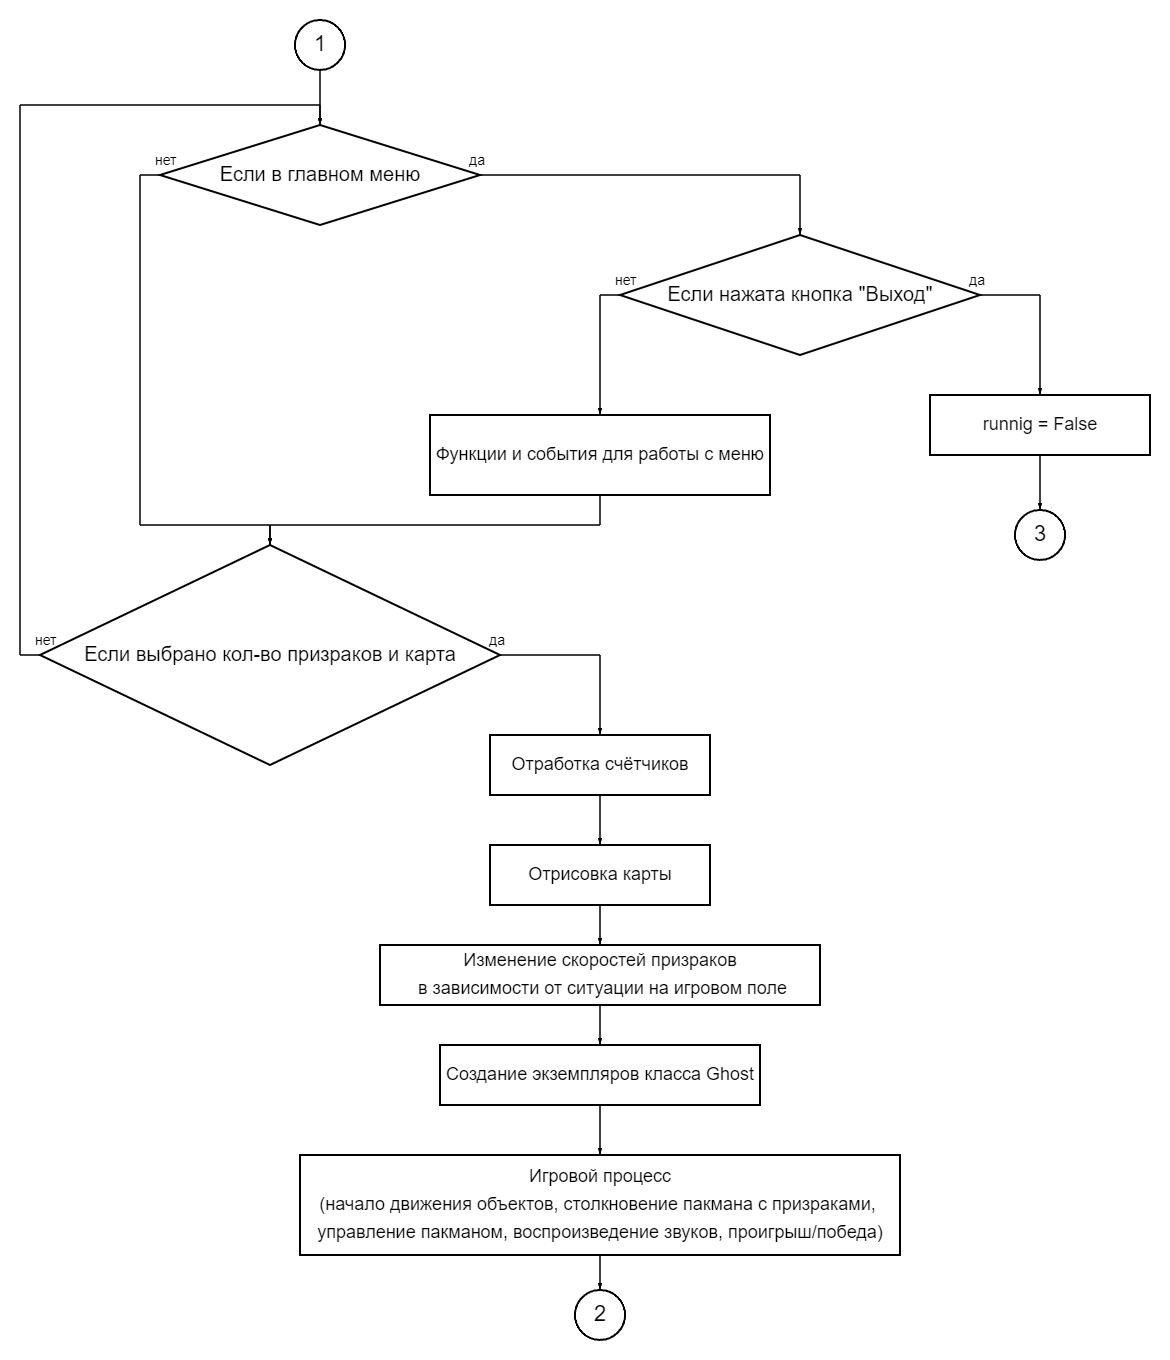
\includegraphics[width=1\linewidth]{images/flow2.png}
	\caption{Блок-схема алгоритма программы.}
	\label{fig8}
\end{figure}

\subsection{\label{subsec:ch02/sec01/sub09}Сборка программы.}
\textbf{PyInstaller} объединяет приложение Python и все его зависимости в один пакет~\cite{pyinstEN}. Пользователь может запустить упакованное приложение без установки интерпретатора Python или каких-либо модулей. PyInstaller поддерживает Python 3.8 и новее и правильно объединяет многие основные пакеты Python, такие как numpy, matplotlib, PyQt, wxPython и другие. PyInstaller протестирован на Windows, MacOS X и Linux.

Так как для разработки была выбрана ОС Microsfot Windows, то сборка игры выполнялась под неё. Аналогичные действия можно выполнить и для ОС GNU/Linux.
Для преобразования python-файла в испольняемый файл .exe нужно было выполнить следующую команду в командной строке Windows: \textsl{pyinstaller --onefile --noconsole main.py}. В итоге получаем несколько папок и сам exe-файл. Чтобы файл успешно запустился, его нужно поместить в одну директорию с папкой Source, которая содержит шрифт, текстуры и звуки, необходимые для игры, а также скопировать туда dll-файлы библиотеки PySDL2. В итоге директория будет иметь вид (см. рисунок~\ref{fig9}).
\begin{figure}[H]
	\centering
	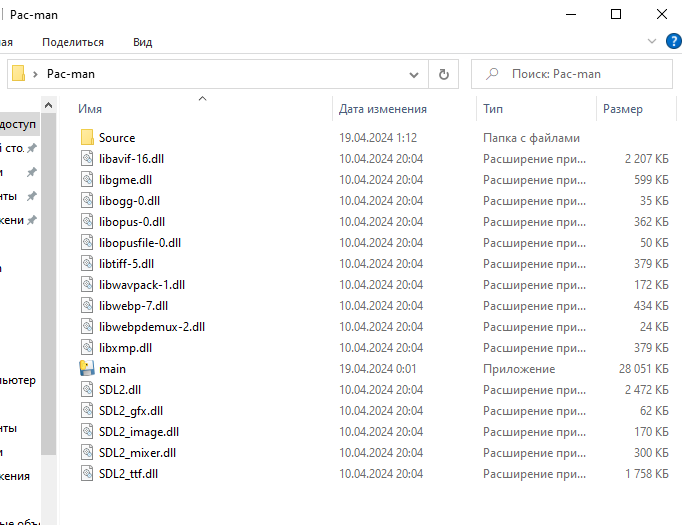
\includegraphics[width=1\linewidth]{images/dir.png}
	\caption{Директория с исполняемым файлом.}
	\label{fig9}
\end{figure}
После нескольких запусков сборки у разных пользователей ОС Windows было обнаружено, что exe-файл не запускается, потому что его блокирует либо встроенный защитник Windows, либо сторонний антивирус. Решается эта проблема легко: нужно либо отключить защиту, либо добавить файл в исключения.

\section{\label{sec:ch02/sec02}Проверка работоспособности программы.}
При запуске игры нас встречает главное меню (см. \textbf{\textsc{ПРИЛОЖЕНИЕ}} на стр.~\pageref{fig2}).

При нажатии на кнопку <<Помощь>> меняется экран. На нём отображена инфорамация в соответствии с ТЗ (см. \textbf{\textsc{ПРИЛОЖЕНИЕ}} на стр.~\pageref{fig3}).

При нажатии на кнопку <<Начать игру>> меняется экран. На нём отображены кнопки выбора количества призраков и карты в соответствии с ТЗ (см. \textbf{\textsc{ПРИЛОЖЕНИЕ}} на стр.~\pageref{fig4}).

Для примера описанного выше (см. \textbf{\textsc{Главная функция игры}} на стр.~\pageref{subsec:ch02/sec01/sub07}) игровое поле выглядит следующим образом (см. \textbf{\textsc{ПРИЛОЖЕНИЕ}} на стр.~\pageref{fig5}).

Пример ситуации, когда пакман потерял одну жизнь, некоторые призраки испуганы, съедены (глаза) и перерождены приведены ниже (см. \textbf{\textsc{ПРИЛОЖЕНИЕ}} на стр.~\pageref{fig6}). 

\chapter*{Заключение}
\phantomsection\addcontentsline{toc}{chapter}{ЗАКЛЮЧЕНИЕ}
В ходе выполнения лабораторной работы была создана кроссплатформенная программа с использованием языка программирования Python3 и библиотеки PySDL2.

Программа создавалась в объектно-ориентированной парадигме.

Программа представляет собой аркадную игру Pac-man.

Кнопки, экраны <<Помощь>> и <<Начать игру>>, пакман, призраки, точки, карты -- все эти объекты были добавлены в программу. Кнопки срабатывают при нажатии на них, при этом меняется экран. Выбор карты и количества призраков успешно выполняется. Пакман управляется стрелками, призраки гоняются за ним. Все взаимодействия между пакманом, точками, призраками и лабиринтом успешно отрабатываются. 

Программы выполнена в соответствии с \textbf{\textsc{Техническим заданием}} на странице~\pageref{sec:ch01/sec01}.

Были решены все поставленные задачи (см. \textbf{\textsc{Задачи}} на стр.~\pageref{zadachi}).

Разработка программы и отчёта производилась с использованием системы контроля версий Git, а именно с помощью онлайн-хранилища GitHub.

По коду программы была создана блок-схема (см. на стр.~\pageref{fig7}~\pageref{fig8}).

Проверка работоспособности программы была проведена успешно (см. \textbf{\textsc{Проверка работоспособности программы}} на стр.~\pageref{sec:ch02/sec02}).

Отчёт оформлен с помощью системы компьютерной вёрстки \TeX{} и его расширения \XeTeX{} из дистрибутива \textit{TeX Live}.

Ссылка на репозиторий проекта:~\textcolor{blue}{\url{https://github.com/davyd-off/Pac-man}}

\newpage
\phantomsection\addcontentsline{toc}{chapter}{СПИСОК ИСПОЛЬЗОВАННОЙ ЛИТЕРАТУРЫ}
\printbibliography[title={Список использованной литературы}]

\appendix
\newpage
\chapter*{\raggedleft\label{appendix1}Приложение}
\addcontentsline{toc}{chapter}{Приложение}

\begin{code}
	\captionof*{listing}{Главный файл игры Pac-Man на языке \textit{Python} с использованием библиотеки \textit{PySDL2}~\pageref{pysdl2}.}\label{code:main}
	\inputminted[mathescape,linenos,frame=lines,fontsize=\tiny,breaklines]{Python}{src/main.py}
\end{code}

\begin{code}
	\captionof*{listing}{Файл игры Pac-Man на языке \textit{Python}, содержащий класс для создания игрового меню.}\label{code:menu}
	\inputminted[mathescape,linenos,frame=lines,fontsize=\tiny,breaklines]{Python}{src/button.py}
\end{code}

\begin{code}
	\captionof*{listing}{Файл игры Pac-Man на языке \textit{Python}, содержащий двумерный массив, по которому отрисовывается 1 карта.}\label{code:b1}
\inputminted[mathescape,linenos,frame=lines,fontsize=\tiny,breaklines]{Python}{src/board_1.py}
\end{code}

\begin{code}
	\captionof*{listing}{Файл игры Pac-Man на языке \textit{Python}, содержащий двумерный массив, по которому отрисовывается 2 карта.}\label{code:b2}
\inputminted[mathescape,linenos,frame=lines,fontsize=\tiny,breaklines]{Python}{src/board_2.py}
\end{code}

\begin{code}
	\captionof*{listing}{Файл игры Pac-Man на языке \textit{Python}, содержащий двумерный массив, по которому отрисовывается 3 карта.}\label{code:b3}
\inputminted[mathescape,linenos,frame=lines,fontsize=\tiny,breaklines]{Python}{src/board_3.py}
\end{code}

\begin{code}
	\captionof*{listing}{Файл игры Pac-Man на языке \textit{Python} для отрисовки карты.}\label{code:level}
\inputminted[mathescape,linenos,frame=lines,fontsize=\tiny,breaklines]{Python}{src/level.py}
\end{code}

\begin{code}
	\captionof*{listing}{Файл игры Pac-Man на языке \textit{Python} с функциями пакмана.}\label{code:player}
	\inputminted[mathescape,linenos,frame=lines,fontsize=\tiny,breaklines]{Python}{src/player.py}
\end{code}

\begin{code}
	\captionof*{listing}{Файл игры Pac-Man на языке \textit{Python}, содержащий класс для создания призраков.}\label{code:ghost}
	\inputminted[mathescape,linenos,frame=lines,fontsize=\tiny,breaklines]{Python}{src/ghost.py}
\end{code}

\begin{figure}[H]
	\centering
	
\includegraphics[width=1\linewidth]{images/1.png}
	\caption{Главное меню игры.}
	\label{fig2}
\end{figure}

\begin{figure}[H]
	\centering
	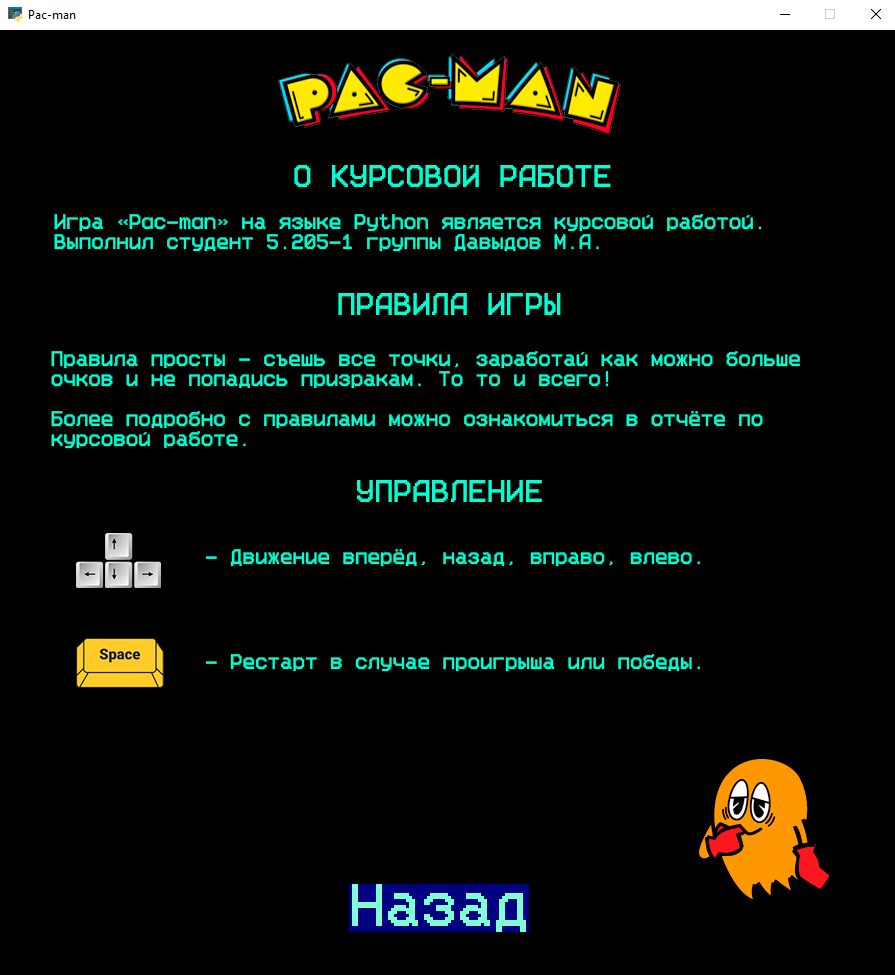
\includegraphics[width=1\linewidth]{images/2.png}
	\caption{Раздел <<Помощь>>.}
	\label{fig3}
\end{figure}

\begin{figure}[H]
	\centering
	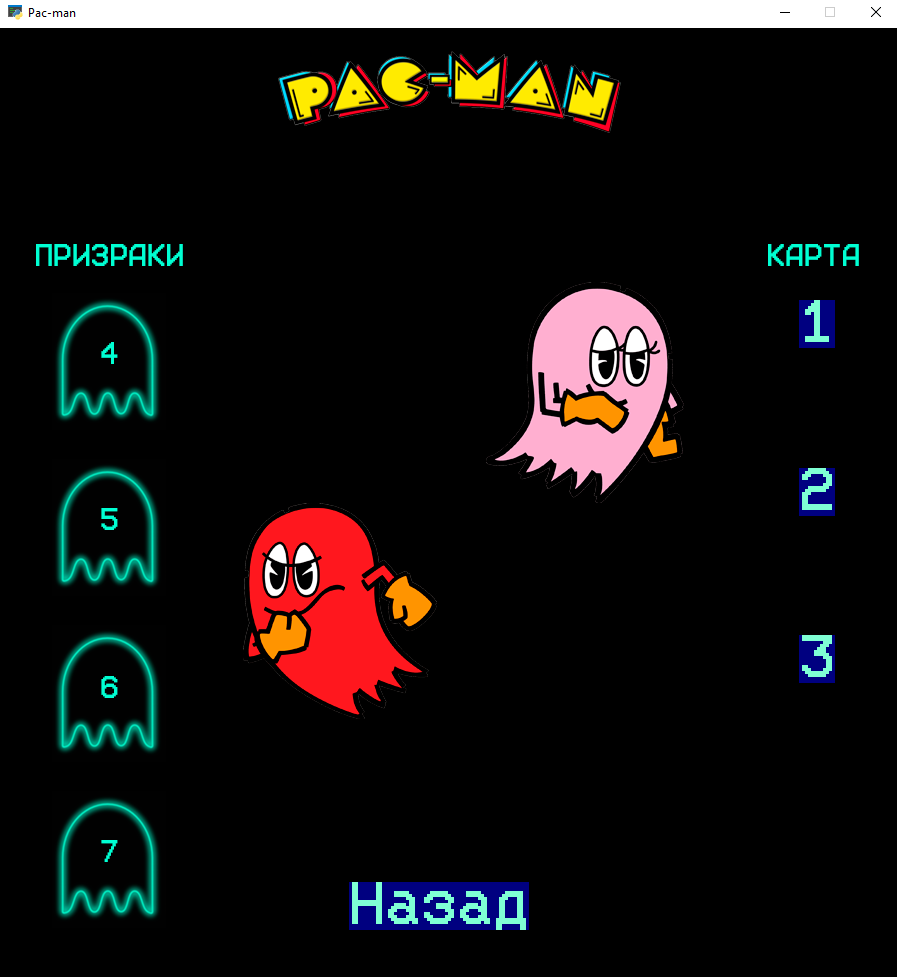
\includegraphics[width=1\linewidth]{images/3.png}
	\caption{Раздел <<Начать игру>>.}
	\label{fig4}
\end{figure}

\begin{figure}[H]
	\centering
	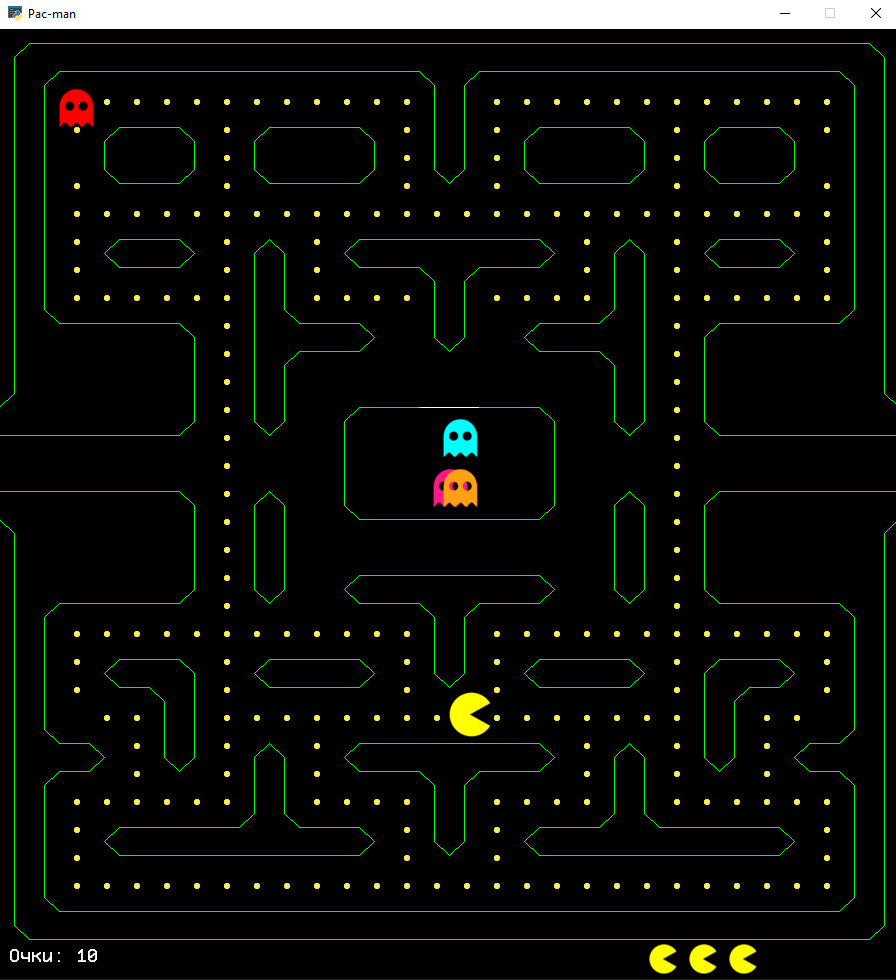
\includegraphics[width=1\linewidth]{images/4.png}
	\caption{Начальное игровое поле для 1-ой карты и 4-ёх призраков.}
	\label{fig5}
\end{figure}

\begin{figure}[H]
	\centering
	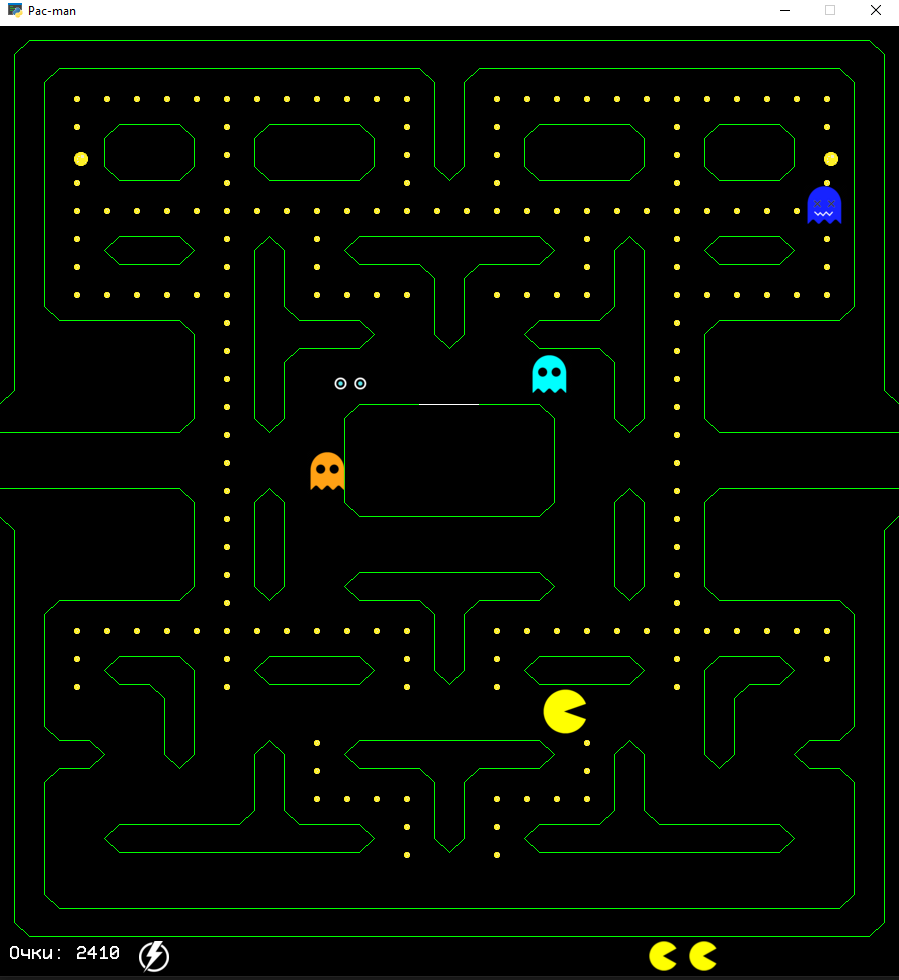
\includegraphics[width=1\linewidth]{images/5.png}
	\caption{Пример ситуации.}
	\label{fig6}
\end{figure}

\end{document}

